%----------------------------------------------------------------------------------------
%   Доорх хэсгийг өөрчлөх шаардлагагүй
%----------------------------------------------------------------------------------------
% !TEX TS-program = xelatex
% !TEX encoding = UTF-8 Unicode
\documentclass[12pt,a4paper]{report}

% \usepackage{fontspec,xltxtra,xunicode}
% \usepackage{fontspec}
% \setmainfont{Times New Roman}
% \setsansfont{Arial}

% \usepackage[T2A]{fontenc}
% \usepackage[utf8]{inputenc}
% \usepackage[english, mongolian]{babel}

\usepackage{polyglossia}
\setmainlanguage{mongolian}
\setotherlanguage{english}
\setmainfont{Times New Roman}
\setsansfont{Arial}
\setromanfont{Times New Roman} 
\newfontfamily{\cyrillicfont}{Times New Roman}[Ligatures=TeX]
\newfontfamily{\cyrillicfontrm}{Times New Roman}
\newfontfamily{\cyrillicfonttt}{Courier New}
\newfontfamily{\cyrillicfontsf}{Arial}
\setkeys{mongolian}{babelshorthands=true}

%\usepackage{natbib}
\usepackage{geometry}
%\usepackage{fancyheadings} fancyheadings is obsolete: replaced by fancyhdr. JL
\usepackage{fancyhdr}
\usepackage{float}
\usepackage{afterpage}
\usepackage{graphicx}
\usepackage{amsmath,amssymb,amsbsy}
\usepackage{dcolumn,array}
\usepackage{tocloft}
\usepackage{dics}
\usepackage{nomencl}
\usepackage{upgreek}
\newcommand{\argmin}{\arg\!\min}
\usepackage{mathtools}
\usepackage[hidelinks, unicode]{hyperref}
\pdfstringdefDisableCommands{\let\uppercase\relax}

\usepackage{algorithm}
\usepackage{algpseudocode}

\usepackage{listings}
\DeclarePairedDelimiter\abs{\lvert}{\rvert}%
\makeatletter
\usepackage{subcaption}
\usepackage[justification={centering}]{caption}
\captionsetup[table]{belowskip=0.5pt}
\usepackage{subfiles}
\usepackage[bottom]{footmisc}
\usepackage{listings}
\renewcommand{\lstlistingname}{Код}
\renewcommand{\lstlistlistingname}{\lstlistingname ын жагсаалт}
\usepackage[final]{pdfpages}

\usepackage{color}
\definecolor{codegreen}{rgb}{0,0.6,0}
\definecolor{codegray}{rgb}{0.5,0.5,0.5}
\definecolor{codepurple}{rgb}{0.58,0,0.82}
\definecolor{backcolour}{rgb}{0.99,0.99,0.99}
 
\lstdefinestyle{mystyle}{
    basicstyle=\ttfamily\small,
    backgroundcolor=\color{backcolour},   
    commentstyle=\color{codegreen},
    keywordstyle=\color{magenta},
    numberstyle=\tiny\color{codegray},
    stringstyle=\color{codepurple},
    %basicstyle=\footnotesize,
    breakatwhitespace=false,
    breaklines=true,
    captionpos=b,
    keepspaces=false,
    numbers=left,
    numbersep=10pt,
    showspaces=false,
    showstringspaces=false,
    showtabs=false,
    tabsize=2
}
 
\lstset{style=mystyle, label=DescriptiveLabel} 

 %define Javascript language
 \lstdefinelanguage{JavaScript}{
	keywords={typeof, new, true, false, catch, function, return, null, catch, switch, var, if, in, while, do, else, case, break},
	keywordstyle=\color{blue}\bfseries,
	ndkeywords={class, export, boolean, throw, implements, import, this},
	ndkeywordstyle=\color{darkgray}\bfseries,
	identifierstyle=\color{black},
	sensitive=false,
	comment=[l]{//},
	morecomment=[s]{/*}{*/},
	commentstyle=\color{purple}\ttfamily,
	stringstyle=\color{red}\ttfamily,
	morestring=[b]',
	morestring=[b]"
	}
	 
	\lstset{
	language=JavaScript,
	extendedchars=true,
	basicstyle=\footnotesize\ttfamily,
	showstringspaces=false,
	showspaces=false,
	numbers=left,
	numberstyle=\footnotesize,
	numbersep=9pt,
	tabsize=2,
	breaklines=true,
	showtabs=false,
	captionpos=b
	}

\let\oldabs\abs
\def\abs{\@ifstar{\oldabs}{\oldabs*}}
\makenomenclature
\begin{document}


%----------------------------------------------------------------------------------------
%   Өөрийн мэдээллээ оруулах хэсэг
%----------------------------------------------------------------------------------------

% Дипломийн ажлын сэдэв
\title{МЭДЭЭЛЛИЙН ЭХ СУРВАЛЖАА ХУВААЛЦАХ СОШИАЛ ПЛАТФОРМ}
% Дипломын ажлын англи нэр
\titleEng{Information sources sharing social platform}
% Өөрийн овог нэрийг бүтнээр нь бичнэ
\author{Батбаярын Бат-Өлзий}
% Өөрийн овгийн эхний үсэг нэрээ бичнэ
\authorShort{Б. Бат-Өлзий}
% Удирдагчийн зэрэг цол овгийн эхний үсэг нэр
\supervisor{Мастер Р. Жавхлан}
% Хамтарсан удирдагчийн зэрэг цол овгийн эхний үсэг нэр
% \cosupervisor{Др. Г.Амарсанаа}

% СиСи дугаар 
\sisiId{18B1NUM3474}
% Их сургуулийн нэр
\university{МОНГОЛ УЛСЫН ИХ СУРГУУЛЬ}
% Бүрэлдэхүүн сургуулийн нэр
\faculty{ХЭРЭГЛЭЭНИЙ ШИНЖЛЭХ УХААН, ИНЖЕНЕРЧЛЭЛИЙН СУРГУУЛЬ}
% Тэнхимийн нэр
\department{МЭДЭЭЛЭЛ, КОМПЬЮТЕРИЙН УХААНЫ ТЭНХИМ}
% Зэргийн нэр
\degreeName{Бакалаврын судалгааны ажил}
% Суралцаж буй хөтөлбөрийн нэр
\programeName{Програм Хангамж (D 061302)}
% Хэвлэгдсэн газар
\cityName{Улаанбаатар}
% Хэвлэгдсэн огноо
\gradyear{2022 он}


%----------------------------------------------------------------------------------------
%   Доорх хэсгийг өөрчлөх шаардлагагүй
%----------------------------------------------------------------------------------------
%----------------------Нүүр хуудастай хамаатай зүйлс----------------------------
\pagenumbering{roman}
\makefrontpage
\maketitle

\doublespace

% Decleration
\begin{huge}
	\textbf{Зохиогчийн баталгаа}
\end{huge} \\ \ \\
\doublespace
Миний бие \@author \ "\@title" \ сэдэвтэй судалгааны ажлыг гүйцэтгэсэн болохыг зарлаж дараах зүйлсийг баталж байна:
\begin{itemize}
	\item Ажил нь бүхэлдээ эсвэл ихэнхдээ Монгол Улсын Их Сургуулийн зэрэг горилохоор дэвшүүлсэн болно.
	\item Энэ ажлын аль нэг хэсгийг эсвэл бүхлээр нь ямар нэг их, дээд сургуулийн зэрэг горилохоор оруулж байгаагүй.
	\item Бусдын хийсэн ажлаас хуулбарлаагүй, ашигласан бол ишлэл, зүүлт хийсэн.
	\item Ажлыг би өөрөө (хамтарч) хийсэн ба миний хийсэн ажил, үзүүлсэн дэмжлэгийг дипломын ажилд тодорхой тусгасан.
	\item Ажилд тусалсан бүх эх сурвалжид талархаж байна.
\end{itemize}
\

Гарын үсэг: \underline{\hspace{5cm}}

Огноо: 	\ \ \underline{\hspace{3cm}}

% Гарчгийг автоматаар оруулна
\setcounter{tocdepth}{1}
\tableofcontents

% Зургийн жагсаалтыг автоматаар оруулна
\addcontentsline{toc}{part}{ЗУРГИЙН ЖАГСААЛТ}
\listoffigures

% Хүснэгтийн жагсаалтыг автоматаар оруулна
\addcontentsline{toc}{part}{ХҮСНЭГТИЙН ЖАГСААЛТ}
\listoftables

% Кодын жагсаалтыг автоматаар оруулна
\addcontentsline{toc}{part}{КОДЫН ЖАГСААЛТ.}
\lstlistoflistings

% This puts the word "Page" right justified above everything else.
\newpage
\addtocontents{lof}{Зураг~\hfill Хуудас \par}

\renewcommand{\cftlabel}{Зураг}

\doublespace
\pagenumbering{arabic}


\begin{abstract}
Орчин цагт интернэт сүлжээ хүмүүсийн амьдралын салшгүй нэг хэсэг болж түүнийгээ дагаад бүхий л мэдээ мэдээллийг интернэт дэх нэмэлт эх сурвалжуудаас авдаг болсон. Аливаа зүйлс томрох тусам найдвартай, чанартай зүйлстэй зэрэгцэн худал хуурмаг зүйлс их тархдаг билээ. Үүнтэй ижлээр хүмүүс интернэт дэх хэт олон эх сурвалжууд дунд төөрч, хэрэгцээгүй мэдээлэл унших, түүнийгээ бусдад хуваалцаж бусдыг болон өөрсдийгөө үргэлжлүүлэн хохироосоор байна. Үүнээс авч үзвэл интернэт хэрэглэгчид мэргэжлийн хүмүүсийн цуглуулсан чанартай агуулгатай эх сурвалжуудыг хялбар, нэгдсэн байдлаар харах, мөн өөрөө эх сурвалжуудаа цуглуулж бусдад хуваалцах шаардлага тулгарч байна.

	\setcounter{secnumdepth}{0}

  \section{Зорилго}
	Мэдээллийн эх сурвалжуудаа нэгтгэж бусдад хуваалцах, бусдын цуглуулсан эх сурвалжуудыг хялбар байдлаар харах, үнэлгээ өгөх боломжтой веб апп бүтээж интернэт хэрэглэгчдийн нэмэлт эх сурвалж олох явцыг хялбаршуулахаар зорьж байна.

	\section{Зорилт}
	Уг веб аппыг хөгжүүлэхдээ дараах үе шатын дагуу ажиллана.
	\begin{enumerate}
		\item Хэрэглэгчийн үндсэн шаардлагуудыг тодорхойлох
		\item UX судалгаа хийж хэрэглэгч суурьтай хялбар интерфейс дизайн гаргах
		\item Ашиглах технологийг онол болон практик дээр суурилж судлах, 
		\item Системийн архитектурыг зохион байгуулж бэлдэх
		\item Гаргасан баримт бичиг дээрээ тулгуурлаж хөгжүүлэлтээ хийх
		\item Эцсийн хэрэглэгчиддээ зориулж бүтээгдэхүүн болгон гаргах
	\end{enumerate}
	
	\section{Сэдэв сонгох үндэслэл}

	2022 оны 4-р сарын байдлаар дэлхийн нийт хүм амын 63.1 хувь буюу ойролцоогоор 5 тэрбум хүн интернэт сүлжээг хэрэглэдэг ба үүнээс 4.7 тэрбум хүн буюу 94 хувь нь өдөр тутмын амьдралдаа сошиал сүлжээг ашиглаж бусадтай харилцах, мэдээ мэдээллээ авах хэрэгцээгээ хангадаг байна \footnote{Дэлхийн интернэт хэрэглэгчдийн судалгаа: \url{https://www.statista.com/statistics/617136/digital-population-worldwide/}}. Өөрөөр хэлбэл дэлхийн хүн амын талаас их хувь нь хэвмэлэл биет материал, телевиз, радиогоос гадна нэмэлтээр интернэт дэх веб холбоосуудаар дамжин нэмэлт мэдээллээ авдаг гэсэн үг билээ.
	
	Миний хувьд сошиал сүлжээ ашиглан уг сэдэвтэй холбоотой судалгааг\footnote{Эх сурвалжтай холбоотой судалгаа: \url{https://docs.google.com/spreadsheets/d/1CfVnHT29pkBiL0JBv7bXiKtOxERQfTzt0PmOaQ-mcd0/edit?usp=sharing}} 58 интернэт хэрэглэгчдээс авсан бөгөөд тэдгээрт тулгарсан асуудлууд болон хариултуудыг дүгнэж үзвэл

	\begin{figure}[h]
		\centering
		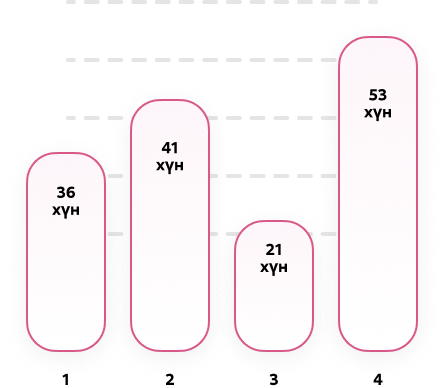
\includegraphics[width=5cm]{images/statistic.png}
		\caption{Интернэт хэрэглэгчдээс авсан судалгааны үр дүн}
		\label{fig:results}
	\end{figure}

	\begin{enumerate}
		\item Маш олон хуурамч мэдээллүүдэд өртдөг - 36 хүн
		\item Өөрт хэрэгтэй мэдээллээ олоход цаг их зарцуулдаг - 41 хүн
		\item Сэдвийнхээ хүрээнд өөрийн олж авсан эх сурвалжуудын тоонд сэтгэл хангалуун бус байдаг - 21 хүн
		\item Ном, зурагтаас илүү интернэт ашиглан мэдээллээ авдаг - 53 хүн
	\end{enumerate}

	гэсэн хариу гарсан. Иймд эдгээр болон бусад хэрэглэгчдэд шаардлагатай зөвхөн эх сурвалжуудаа олж авах, бусдад хуваалцах боломжтой сошиал платформыг бүтээсэн нь зөв гэж үзсэн тул уг сэдвийг сонгон хөгжүүлж байна.

	\section{Ач холбогдол}
	Уг платформыг бүтээснээр миний хувьд бүтээгдэхүүнийг эхнээс нь дуусах хүртэлх хөгжүүлэлтийн үе шатуудтай танилцах, түүнийгээ практикаар хэрэгжүүлэх боломж бүрдэнэ. 

	Мөн бүтээгдэхүүн болгон гаргаж хэрэглээнд нэвтрүүлснээр дээр дурдсан асуудлыг тодорхой хэмжээнд багасах боломжтой гэж үзэж байна. Маш олон төрлөөр хэрэглэх боломжтой ба жишээ нь их сургуулийн багш оюутнууддаа зориулж сэдвийн хүрээнд нэмэлт материал бэлдэхдээ интернэт сүлжээнд байрласан унших ёстой судалгааны ажил, үзэх ёстой бичлэг, дагаж хийх ёстой практик хичээлүүдийнхээ веб холбоосуудыг хялбар байдлаар нэгтгэж, хуваалцах боломж бүрдэх юм. Мөн багш нь өөрийн сонирхдог сэдвийн хүрээнд бусдын оруулсан эх сурвалжуудтай танилцах боломжтой. 
	\setcounter{secnumdepth}{2}
	% \thispagestyle{plain}

\end{abstract}


\addcontentsline{toc}{part}{БҮЛГҮҮД}

\subfile{chapters/research.tex}
\subfile{chapters/requirement.tex}
\subfile{chapters/architecture.tex}
\subfile{chapters/implementation.tex}
% \subfile{chapters/result.tex}


\chapter{Дүгнэлт}

Энэхүү судалгааны ажлаар орчин үеийн дижитал бүтээгдэхүүний хөгжүүлэлтийн арга барилтай танилцаж хэрэглэгчийн шаардлагыг тодорхойлохоос эхлээд UX судалгаа хийж хэрэглэгч төвтэй интерфэйс дизайн гаргах, шинэлэг технологиудыг ашиглан хөгжүүлэлтийг гүйцэтгэж, өөрийн санаагаа бүрэн ажиллагаатай, хүмүүсийн асуудлыг шийдвэрлэж чадсан сошиал платформ болгож чадсан нь өөрт маань их хэмжээний мэдлэг, туршлага болж үлдсэн гэдэгт итгэлтэй байна.

Мөн цаашлаад уг сошиал платформыг эхний түвшинд Монгол Улсын Их Сургуулийн SISI системийн OAuth-г нэвтрүүлж багш, оюутнууд хоорондоо мэдээллийн эх сурвалжаа хялбар байдлаар хуваалцах, хичээлээс гадуур нэмэлт эх сурвалжыг олох явдлыг хялбаршуулах боломжтой туслах систем болгон хөгжүүлэх бүрэн боломжтой гэж үзэж байна.

\renewcommand\bibname{Ашигласан материал}
\addcontentsline{toc}{part}{НОМ ЗҮЙ}


\appendix
\renewcommand\bibname{Хавсралт}
\addcontentsline{toc}{part}{ХАВСРАЛТ}

\chapter{Prisma модел}
\label{appendix:prisma-model}

\begin{lstlisting}[language=Javascript, frame=single]
	generator client {
		provider = "prisma-client-js"
		previewFeatures = ["interactiveTransactions"]
	}
	
	datasource db {
		provider = "postgresql"
		url      = env("DATABASE_URL")
		shadowDatabaseUrl = env("SHADOW_DATABASE_URL")
	}
	
	model User {
		id         Int    @id @default(autoincrement())
		username   String
		email      String
		password   String
		profileImg String
	
		followers Follows[] @relation("following")
		following Follows[] @relation("follower")
		votes Votes[] @relation("userVotes")
	
		posts Post[]
		createdAt DateTime @default(now())
		updatedAt DateTime @updatedAt
	}
	
	model Post {
		id       Int    @id @default(autoincrement())
		ogUrl    String
		ogTitle  String
		ogImage  String
		authorId Int
		author   User   @relation(fields: [authorId], references: [id], onDelete: Cascade)
		groupId  Int?
		group    Group? @relation(fields: [groupId], references: [id])
	
		votes Votes[] @relation("postVotes")
	
		tags       Tag[]
		categories Category[]
	
		createdAt DateTime @default(now())
		updatedAt DateTime @updatedAt
	}
	
	model Tag {
		id   Int    @id @default(autoincrement())
		name String
	
		posts Post[]
	
		createdAt DateTime @default(now())
		updatedAt DateTime @updatedAt
	}
	
	model Category {
		id   Int    @id @default(autoincrement())
		name String
	
		posts Post[]
	
		createdAt DateTime @default(now())
		updatedAt DateTime @updatedAt
	}
	
	model Group {
		id          Int    @id @default(autoincrement())
		title       String
		description String
	
		createdAt DateTime @default(now())
		updatedAt DateTime @updatedAt
		Post      Post[]
	}
	
	model Follows {
		follower    User @relation("follower", fields: [followerId], references: [id])
		followerId  Int
		following   User @relation("following", fields: [followingId], references: [id])
		followingId Int
	
		@@id([followerId, followingId])
	
		createdAt DateTime @default(now())
	}
	
	model Votes {
		id          Int    @id @default(autoincrement())
		user User @relation("userVotes",fields: [userId], references: [id])
		userId Int
		post Post @relation("postVotes",fields:[postId],references:[id])
		postId Int
		vote String
	
		createdAt DateTime @default(now())
		updatedAt DateTime @updatedAt
		deletedAt DateTime?
	}
\end{lstlisting}

\chapter{Prisma Client ашиглах}
\label{appendix:prisma-client}

\begin{lstlisting}[language=Javascript, frame=single]
	import { PrismaClient } from '@prisma/client'

	let prisma: PrismaClient
	
	if (process.env.NODE_ENV === 'production') {
		prisma = new PrismaClient()
	} else {
		if (!global.prisma) {
			global.prisma = new PrismaClient()
		}
		prisma = global.prisma
	}
	
	export default prisma
\end{lstlisting}

\chapter{Next.js дээр remote домайн зөвшөөрөх}
\label{appendix:next-config}

\begin{lstlisting}[language=Javascript, frame=single]
	@type {import('next').NextConfig}
	const nextConfig = {
		reactStrictMode: true,
		images: {
			remotePatterns: [
				{
					protocol: "https",
					hostname: "**",
				},
				{
					protocol: "http",
					hostname: "**",
				},
			],
		},
	};
	
	module.exports = nextConfig;
	
\end{lstlisting}

\chapter{Tailwind custom-class үүсгэх}
\label{appendix:custom-class}

\begin{lstlisting}[language=Javascript, frame=single]
	@tailwind base;
	@tailwind components;
	@tailwind utilities;
	
	@layer components {
		.sidebar-icon {
			@apply flex h-10 w-10 cursor-pointer items-center justify-center rounded-lg transition-all duration-75 hover:border-2 hover:border-primary;
		}
	
		.sidebar-icon-active {
			@apply flex h-10 w-10 cursor-pointer items-center justify-center rounded-lg border-2 border-primary bg-white hover:bg-gray100;
		}
	
		.tooltip {
			@apply absolute left-14 z-10 m-2 w-auto min-w-max origin-left scale-0 rounded-md bg-gray-900 p-2 text-xs font-bold text-white shadow-md transition-all duration-100;
		}
	
		.vote-btn {
			@apply grid h-8 w-8 cursor-pointer place-content-center rounded-lg border border-gray200 bg-white hover:border-gray100;
		}
	
		.bar {
			@apply z-0 my-1 flex justify-between px-5 py-3 text-sm text-description transition-all duration-100 hover:text-black;
		}
	
		.chip {
			@apply flex h-5 items-center rounded-md border border-gray100 bg-gray300 px-1 text-xs;
		}
	
		.bar-active {
			@apply relative z-0 my-1 flex justify-between px-5 py-3 text-sm transition-all duration-100 hover:text-black;
		}
	
		.chip-active {
			@apply flex h-5 items-center rounded-md bg-black px-1 text-xs text-white;
		}
	}
	
\end{lstlisting}

\chapter{Хэрэглэгчийн мэдээллийг гаргах endpoint}
\label{appendix:user-post-endpoint}

\begin{lstlisting}[language=Javascript, frame=single]
	import { NextApiRequest, NextApiResponse } from "next";
	import prisma from "../../../../lib/prisma";
	
	export default async function handle(req: NextApiRequest, res: NextApiResponse) {
		try {
			
			const uId = parseInt(req.query.id as string, 10)
			
			const resultDB = await prisma.user.findUnique({
				where: {
					id: uId
				},
				select: {
					id: true,
					username: true,
					profileImg: true,
					posts: {
						select: {
							id: true,
							ogUrl: true,
							ogTitle: true,
							ogImage: true,
							tags: true,
							group: true,
						},
					}
				}
			})
	
			res.status(200).json(resultDB);
		} catch (err) {
			res.status(403).json({ err: "Error occured"})
		}
	}
\end{lstlisting}

\chapter{Холбоос дээр Vote өгөх endpoint}
\label{appendix:user-vote-endpoint}

\begin{lstlisting}[language=Javascript, frame=single]
	import {NextApiRequest, NextApiResponse} from "next";
	import {Prisma} from "@prisma/client";
	import {instanceOf} from "prop-types";
	import prisma from "../../../../lib/prisma";
	
	
	export default async function handle(req: NextApiRequest, res: NextApiResponse) {
			const requestMethod = req.method
			switch (requestMethod){
					case 'GET':
							let following;
							try{
									let postId = parseInt(req.query.id as string, 10)
									const totalVote = await VotesTotal(postId)
									res.status(200).json({totalVote})
							} catch (e) {
									if (e instanceof Prisma.PrismaClientKnownRequestError) {
											if (e.code === 'P2002') {
													res.json({totalVote:0})
											}else{
													res.status(400).json(e)
											}
									} else {
											console.log(e)
											res.status(500).json({message: "something wrong try again some time later"})
									}
							}
							break
					case 'POST':
							if (req.body.vote!='up'&&req.body.vote!='down'){
									res.status(400)
							}
							let postId = parseInt(req.query.id as string, 10)
							let userId = 1
							let vote = req.body.vote
							await Vote(userId,postId,vote)
							const totalVote = await VotesTotal(postId)
							res.status(200).json({totalVote})
							break
	
					default: res.status(404)
			}
	}
	
	async function Vote(userId:number, postId:number, vote:string){
			return await prisma.$transaction(async (tx) => {
					try {
				const haveVotes = await tx.votes.findFirst({
						where:{
								userId,
								postId,
								deletedAt:null
						},
						orderBy:{
						id:'desc'
						}
				})
					if (haveVotes?.vote==vote){
							return await tx.votes.updateMany({
									where:{
											userId,
											postId,
											deletedAt:null
									},
									data:{
											deletedAt: new Date()
									}
							})
					}else{
							await  tx.votes.updateMany({
									where:{
											userId,
											postId,
											deletedAt:null
									},
									data:{
											deletedAt: new Date()
									}
							})
						 return await tx.votes.create({
									data:{
											user:{
													connect:{
															id: userId
													}
											},
											post: {
													connect:{
															id: postId
													}
											},
											deletedAt: null,
											vote,
									}
							})
					}
					}catch (e) {
							if (e instanceof Prisma.PrismaClientKnownRequestError && e.code == 'P2002') {
									return await tx.votes.create({
											data:{
													user:{
															connect:{
																	id: userId
															}
													},
													post: {
															connect:{
																	id: postId
															}
													},
													deletedAt: null,
													vote,
											}
									})
							}else{
									throw e
							}
					}
					return 1
		})
	}
	
	export function VotesTotal(postId:number){
	
			return  prisma.$transaction(async (tx) => {
					const totalUp = await tx.votes.count({
							where:{
									postId,
									deletedAt:null,
									vote: 'up'
							}
					})
	
					const totalDown = await tx.votes.count({
							where:{
									postId,
									deletedAt:null,
									vote: 'down'
							}
					})
	
					return totalUp-totalDown
			})
	}
	
	async function getLastVote(userID, postID){
			const lastVote = prisma.votes.findFirst({
					where:{
							userId: userID,
							post: postID,
							deletedAt:null
					}
			})
			return lastVote
	}
	
	async function DeletePreviousVotes(userId, postId){
			const res= await prisma.votes.updateMany({
							where:{
									userId,
									postId
							},
							data:{
									deletedAt: new Date()
							}
					}
			)
			return res
	}
	
	async function HaveVotes(userID, postID){
			try {
					const lastVote = await getLastVote(userID,postID)
			}catch (e) {
					if (e instanceof Prisma.PrismaClientKnownRequestError && e.code === 'P2002') {
									return false
					} else {
							throw e
					}
			}
	}
	
\end{lstlisting}

\chapter{Layout компонентийг App компонент дээр ашиглах}
\label{appendix:layout-component}

\begin{lstlisting}[language=Javascript, frame=single]
	import "../styles/globals.css";
	import "../styles/main.css";
	import { Layout } from "../components/Layout";
	import { Rubik } from "@next/font/google";
	
	const rubik = Rubik({
		subsets: ["cyrillic-ext", "cyrillic", "latin", "latin-ext"],
		variable: "--font-rubik",
	});
	
	function MyApp({ Component, pageProps }) {
		return (
			<main className={`${rubik.variable} font-sans`}>
				<Layout>
					<Component {...pageProps} />
				</Layout>
			</main>
		);
	}
	
	export default MyApp;
	
\end{lstlisting}

\end{document}